\section{Transcodificação Assistida por Aprendizado de Máquina}
\label{cap:3.2}

O aprendizado de máquina (do inglês, \textit{Machine Learning}, ML) é um campo de pesquisa que cresceu significativamente nos últimos anos e hoje é aplicado em diversas áreas para resolver diferentes tipos de problema. Na área de codificação de vídeo, isso não é diferente, com contribuições que vão desde o desenvolvimento de novas ferramentas baseadas em aprendizado para codecs híbridos até autoencoders \cite{bib:autoencoder}, codificadores de vídeo totalmente baseados em redes neurais profundas. Quanto às soluções de transcodificação rápida, as propostas são tipicamente focadas em auxiliar as tomadas de decisão, baseando-se em dados extraídos do \textit{bitstream} decodificado e evitando, assim, o teste exaustivo do RDO para várias possibilidades de codificação. Nessas propostas, incluem-se decisões sobre: os modos de predição, a geração de vetores de movimento e a pré-definição de particionamento de blocos. Essa simplificação do processo RDO pode ser tratada como um problema de classificação, pois o modelo treinado poderá detectar: 

\begin{enumerate}[i.]
    \item um modo único a ser testado, descartando todos os restantes;
    
    \item um modo único a ser descartado, testando os demais;
    
    \item um subconjunto de modos a serem testados, descartando os demais.
\end{enumerate}

Algumas soluções de transcodificação assistida por aprendizado de máquina também são baseadas em acelerações locais no lado do codificador, usando modelos treinados com informações obtidas tanto do decodificador (formato de origem) quanto do codificador (formato de destino). Por exemplo, além dos atributos reunidos durante a decodificação, \citet{bib:lucas_2020} também usa a média e a variância dos blocos residuais obtidos durante o processo de codificação do H.266/VVC para prever o particionamento do bloco a ser utilizado. O uso de reaproveitamento de dados de origem tanto do decodificador como do codificador também pode ser observado nos trabalhos de \citet{bib:nguyen_2015}, \citet{bib:franche_2015} e \citet{bib:franche_2017}, apesar de eles não utilizarem soluções baseadas em aprendizado de máquina. Em relação ao conjunto de atributos para serem processados pelo modelo de ML, podem ser diferentes ou idênticos, mesmo para prever decisões distintas. Por exemplo, \citet{bib:peixoto_2014} e \citet{bib:li_2017} usam o mesmo conjunto de recursos em seus trabalhos. Todavia, \citeauthor{bib:peixoto_2014} os usa para prever vetores de movimento a serem utilizados no H.264/AVC, enquanto \citeauthor{bib:li_2017} utiliza esses atributos para prever o particionamento de blocos na codificação H.265/HEVC.

As soluções apresentadas nesses artigos são baseadas em diversos métodos e algoritmos de aprendizado de máquina atualmente disponíveis. As contribuições desses trabalhos na transcodificação de vídeo estão resumidas na Figura \ref{fig:13}, categorizadas de acordo com o algoritmo empregado. No círculo externo da Figura \ref{fig:13}, está a distribuição das categorias de aprendizado de máquina, enquanto, no círculo interno, está a distribuição dos algoritmos utilizados. As soluções observadas na revisão sistemática da literatura se enquadram em três categorias principais de aprendizado de máquina supervisionado \cite{bib:livroKubat}: classificação linear, árvores de decisão e aprendizado profundo, como já foi apresentado na subseção \ref{cap:2.3}.

\begin{figure}
    \centering
    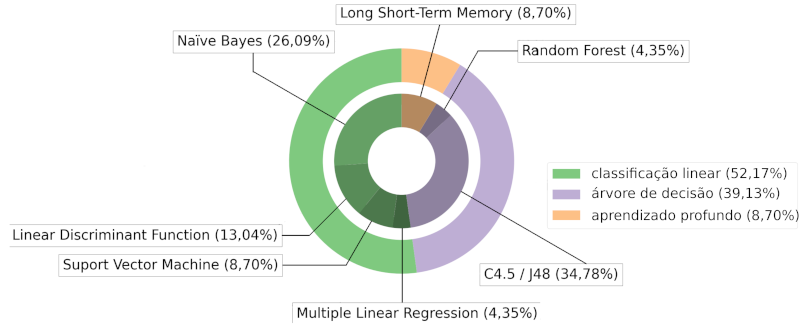
\includegraphics[width=\textwidth]{FIGURES/fig_13.png}
    \caption{Distribuição de algoritmos de aprendizado de máquina nos artigos revisados sobre aceleração de transcodificação de vídeo. Fonte: Elaborada pelo autor.}
    \label{fig:13}
\end{figure}

É possível observar, na Figura \ref{fig:13}, que o algoritmo C4.5/J48, dentro da categoria de árvores de decisão, é o mais empregado nas soluções encontradas na literatura. Por exemplo, \citet{bib:correa_2016} propõe o uso de árvores de decisão treinadas em C4.5 para prever o melhor particionamento de blocos para \textit{Coding Units} (CUs) do H.265/HEVC com base em dados coletados da decodificação do H.264/AVC. Da mesma forma, \citet{bib:escribano3_2008} emprega o mesmo algoritmo de ML para prever vetores de movimento na transcodificação de H.263 para VP6. Já \citet{bib:grellert_2018} usa modelos de \textit{Random Forest} para prever as profundidades máxima e mínima da estrutura de particionamento do H.265/HEVC para acelerar a codificação para aplicativos em tempo real.

Apesar de a categoria de árvores de decisão representar 39,13\% dos trabalhos, não é a mais comum observada na literatura. Conforme a Figura \ref{fig:13}, a categoria de classificadores lineares é a que apresenta maiores contribuições à literatura, totalizando 52,17\% dos trabalhos com uso de aprendizado de máquina. Dentro dessa categoria, \textit{Naïve-Bayes} é o algoritmo mais empregado, seguido por \textit{Linear Discriminant Functions} (LDF), \textit{Support Vector Machine} (SVM) e \textit{Multiple Linear Regression} (MLR). Como já foi dito, esses algoritmos geram modelos classificadores probabilísticos simples e eficientes \cite{bib:naivebayesref} e são amplamente utilizados porque demonstram precisão relevante mesmo para um pequeno conjunto de dados de treinamento. Dentre os trabalhos que fazem uso de \textit{Naïve-Bayes}, temos o de \citet{bib:honrubia_2016}, que propõe um transcodificador H.264/AVC-to-H.265/HEVC que faz uso do modelo para decidir sobre a predição intraquadro e o particionamento de bloco. Estratégia similar é encontrada no trabalho de \citet{bib:li_2017}, ao transcodificar vídeos de VP9 para o padrão H.265/HEVC.

Os últimos algoritmos de aprendizado de máquina que encontramos na literatura revisada se enquadram na categoria de aprendizado profundo. Há poucos trabalhos que implementam soluções a partir deste tipo de algoritmo de aprendizado de máquina, e isso era, de alguma forma, esperado, pois as soluções de aprendizado profundo geralmente exigem recursos computacionais expressivos tanto para o treinamento quanto para sua execução, o que tende a ser contraditório numa proposta de aceleração do transcodificador. Mesmo assim, a abordagem baseada no algoritmo \textit{Long Short-Term Memory} (LSTM) \cite{bib:graves_2012} foi proposta por \citet{bib:xu_2019} para acelerar a transcodificação H.264/AVC-para-H.265/HEVC, levando em consideração vários quadros decodificados do H.264/AVC para predizer sobre o particionamento de blocos do H.265/HEVC e obtendo uma aceleração de 59,6\% no tempo de transcodificação.

Ao utilizar algoritmos de aprendizado de máquina, para realizar a aceleração da transcodificação ou não, é imperativo escolher atributos que representem as informações de modo a auxiliar o modelo a retornar a melhor resposta. Como já vimos nesta seção, os mesmos atributos podem ser utilizados para diferentes fins, e não há consenso sobre quantos ou quais atributos devem ser usados para possibilitar um bom treinamento de modelo. Contudo, de forma genérica, a coleta de um maior número possível de atributos pode ser interessante, cabendo ao algoritmo de aprendizado de máquina decidir quais deles deverão ser levados em consideração durante a previsão. Ao mesmo tempo, é importante ressaltar que o aumento significativo de atributos torna mais complexo o processo de treinamento dos modelos. Ainda assim, considerando todos os artigos revisados que usam estratégias baseadas em aprendizado de máquina, encontramos trabalhos que utilizam menos de uma dezena de atributos e outros que utilizam mais de uma centena.

Para facilitar esse tipo de comparação, apresentamos a Tabela \ref{tab:IV}, que resume a literatura científica que faz uso de modelos de aprendizado de máquina. A Tabela \ref{tab:IV} apresenta ainda o algoritmo de ML utilizado em cada um dos trabalhos destacados na tabela, o estágio da codificação em que foi realizado o reaproveitamento de informação e uma breve descrição dos atributos selecionados. Note que os primeiros nove trabalhos apresentados na Tabela \ref{tab:IV} não fazem parte dos artigos selecionados na revisão sistemática da literatura, pois não apresentam resultados de BD-rate. Todavia, achamos pertinente apresentá-los nesta seção, a fim de possibilitar melhor compreensão do uso de algoritmos de ML em trabalhos de transcodificação de vídeo.

\afterpage{
\clearpage

\begin{landscape}
{\footnotesize
\begin{longtblr}[
    caption = {Resumo das abordagens baseadas em aprendizado de máquina encontradas na literatura para aceleração de transcodificadores de vídeo.},
    label = {tab:IV},
    note{1} = {Este artigo não apresenta resultados de BD-rate.},
    note{2} = {\citet{bib:huangyuan_2015} apresenta resultados de BD-PSNR ao invés de BD-rate.}
]{
    colspec = {p{2.8cm}|p{2cm}|p{3.3cm}|p{1.5cm}|p{13.4cm}},
    rowhead = 1,
    hlines,
    row{even} = {gray9}
}
 \hline
 \textbf{Autor} & \textbf{Algoritmo de ML} & \textbf{Estágios Envolvidos} & \textbf{Número de Atributos} & \textbf{Descrição dos Atributos Utilizados}\\
 
 %2006
 \citet{bib:fernandez2_2006}\TblrNote{1} & J48 & predição interquadros & 292 & Média ($\mu$) e variância ($\sigma^2$) dos blocos residuais de tamanho 4$\times$4; modo de predição no macrobloco (MB); modo de predição interquadros; modo do \textit{Coded Block Pattern} (CBP) do H.262/MPEG-2; modo equivalente ao CBP do H.264/AVC; MB residual quando o vetor de movimentos (VM) do H.262/MPEG-2 é considerado. \\
 
 %2007
 \citet{bib:wang2_2007}\TblrNote{1} & MLR & predição interquadros & 42 & vetores de movimento\\
 
 %2008
 \citet{bib:escribano3_2008}\TblrNote{1} & C4.5 & predição interquadros & 34 & $\mu$ e $\sigma^2$ do bloco residual de tamanho 4$\times$4; VM; modo de predição no MB; CBP. \\
 
 %2008
 \citet{bib:escribano3_2008}\TblrNote{1} & C4.5 & predição interquadros & 12 & $\mu$ e $\sigma^2$ do bloco residual de tamanho 8$\times$8 e 16$\times$16; CBP; erro absoluto quando VM=(0,0). \\
 
 %2008
 \citet{bib:escribano_2008}\TblrNote{1} & C4.5 & predição interquadros & 34 & $\mu$ e $\sigma^2$ do bloco residual de tamanho 4$\times$4; VM; modo de predição no MB; CBP. \\
 
 %2008
 \citet{bib:escribano2_2008}\TblrNote{1} & J48 & predição interquadros & 34 & $\mu$ e $\sigma^2$ do bloco residual de tamanho 4$\times$4; VM; modo de predição no MB; CBP. \\
 
 %2009
 \citet{bib:holder_2009}\TblrNote{1} & J48 & predição interquadros & 291 & $\mu$ e $\sigma^2$ do bloco residual de tamanho 4$\times$4; $\mu$ do bloco residual de tamanho 16$\times$16; CBP; coeficientes da transformada. \\
 
  %2015
 \citet{bib:huangyuan_2015}\TblrNote{2} & SVM & particionamento de blocos & 8 & soma e a $\sigma^2$ dos blocos residuais de tamanho 64$\times$64 e 32$\times$32; soma do bloco residual de tamanho 16$\times$16; modo de predição do MB; tipo de estrutura de particionamento; parâmetro de quantização. \\
 
 %2017
 \citet{bib:wei_2017}\TblrNote{1} & LSTM & particionamento de blocos & 3 & \textit{bitrate}, bloco residual; particionamento do MB. \\
 
 %2014
 \citet{bib:peixoto_2014} & LDF & predição interquadros & 15 & $\sigma^2$ da fase do VM; número de coeficientes da transformada; energia dos coeficientes da transformada; para cada tamanho de CU, sinais de uso do: modo SPLIT, modo SKIP da predição interquadros e do modo 2N$\times$2N da PU. \\
 
 %2014
 \citet{bib:peixoto2_2014} & LDF & particionamento de blocos & 10 & $\sigma^2$ da distância dos VM; $\sigma^2$ da fase do VM; número de coeficientes da transformada; distribuição dos modos de predição do H.264/AVC. \\
 
 %2014
 \citet{bib:honrubia_2014} & NB & particionamento de blocos & 25 & soma, $\mu$ e $\sigma^2$ dos elementos do VM; $\mu$ e $\sigma^2$ da CTU residual; $\mu$ e $\sigma^2$ da CU residual; soma horizontal e vertical dos filtros de Sobel; resolução do vídeo; nível de quantização; \textit{bitrate} da CTU; de cada quadro do vídeo, número de: modos de predição intraquadro, modos SKIP da predição interquadros, predições interquadros no bloco de tamanho 16$\times$16, predições interquadros no bloco de tamanho diferente de 16$\times$16, número de coeficientes da transformada diferente de zero de cada CTU. \\
 
 %2014
 \citet{bib:peixoto3_2014} & LDF & particionamento de blocos & 10 & $\sigma^2$ da distância e das fases do VM; número de coeficientes da transformada; distribuição dos modos de predição do H.264/AVC. \\
 
 %2015
 \citet{bib:honrubia_2015} & NB & particionamento de blocos & 27 & soma, $\mu$ e $\sigma^2$ dos elementos do VM; $\mu$ e $\sigma^2$ da CTU e da CU residual; soma horizontal e vertical dos filtros de Sobel; resolução do vídeo; nível de quantização; \textit{bitrate} da CTU; Lagrangiana do modo SKIP da predição interquadros e dos modos 2N$\times$2N da PU; de cada quadro do vídeo, número de: modos de predição intraquadro, modos SKIP da predição interquadros, predições interquadros no bloco de tamanho 16$\times$16, predições interquadros no bloco de tamanho diferente de 16$\times$16, número de coeficientes da transformada diferente de zero de cada CTU. \\
 
 %2016
 \citet{bib:honrubia_2016} & NB & particionamento de blocos predição intraquadro & 21 & $\mu$ e $\sigma^2$ of residual MB; $\mu$ e $\sigma^2$ of residual CU; number of intra predicted blocks with: horizontal, vertical, diagonal, DC e Planar modes; sum of intra predicted samples within a MB; number of non-zero transform coefficients; video resolution; QP; bitrate; sum of horizontal Sobel Filter; sum of vertical Sobel Filter. \\
 
 %2016
 \citet{bib:correa_2016} & C4.5 & particionamento de blocos & 33 & soma e $\mu$ dos blocos preditos; soma, $\mu$ e número de coeficientes da transformada; sinal de uso do modo SKIP da predição interquadros para os blocos 64$\times$64, 32$\times$32 e 16$\times$16; modo de predição intraquadro para os blocos 64$\times$64, 32$\times$32 e 16$\times$16; modo de predição no MB; CBP dos blocos de crominância. \\
 
 %2017
 \citet{bib:li_2017} & NB & particionamento de blocos & 74 & soma, $\mu$ e $\sigma^2$ dos elementos do VM; custo da taxa-distorção dos modos 2N$\times$2N da PU e dos modos SKIP da predição interquadros; número de blocos dentro de cada superbloco; mapa de profundidade da estrutura de particionamento. \\
 
  %2018
 \citet{bib:liu_2018} & SVM & particionamento de blocos & 3 & $\mu$ do \textit{bitrate}; $\mu$ absoluta dos blocos residuais; número de blocos dentro de cada CTU. \\
 
  %2018
 \citet{bib:grellert_2018} & RF & particionamento de blocos & 19 & modo de predição; modo da PU; profundidade da CU; coeficientes da transformada antes e depois da quantização; soma dos pixeis preditos; magnitude do VM. \\
 
 %2019
 \citet{bib:xu_2019} & LSTM & particionamento de blocos & 12 & VM; bloco residual; particionamento da MB; \textit{bitrate}. \\

 %2019
 \citet{bib:soares_2019} & J48 & particionamento de blocos & 13 & soma e $\mu$ dos coeficientes da transformada; soma e $\mu$ das amostras preditas nos blocos; tipo e posição do MB; CBP das camadas de crominância; sinal de uso do modo SKIP da predição interquadros; sinal de uso de algum modo de predição intraquadro; modo de predição intraquadro usado no bloco de tamanho 16$\times$16. \\
 
  %2019
 \citet{bib:chen_2019} & NB & particionamento de blocos & 3 & profundidade da CU; número de blocos em cada nível de profundidade em cada quadro; número de blocos em cada quadro. \\
 
 %2020
 \citet{bib:lucas_2020} & NB & particionamento de blocos & 16 & $\mu$ e $\sigma^2$ dos coeficientes assimétricos de Fisher e dos coeficientes de Kurtosis nos blocos residuais e reconstruídos para os blocos de tamanho 128$\times$128; $\mu$ das $\sigma^2$ e $\sigma^2$ das $\sigma^2$ dos blocos residuais e reconstruídos para os blocos de tamanho 64$\times$64; número de resíduos iguais a zero dentro do bloco de tamanho 128$\times$128; informação espacial dos blocos residuais de tamanho 128$\times$128; $\mu$ do desvio absoluto entre o bloco residual e o bloco reconstruído; \textit{bitrate}; produto da resolução do vídeo; função lambda entre o nível de quantização utilizado e o valor do grupo de quadros (\textit{group of pictures}, GoP).\\
 \hline
\end{longtblr}
}
\end{landscape}
}


A Tabela \ref{tab:IV} mostra que os artigos revisados empregam diversas informações como atributos. Por exemplo, a média ($\mu$) e a variância ($\sigma^2$) do bloco residual são frequentemente usadas como atributos, como visto em \citet{bib:fernandez2_2006}, \citet{bib:holder_2009}, \citet{bib:huangyuan_2015}, e \citet{bib:honrubia_2015}. Além disso, é possível encontrar atributos baseados em algum tipo de informação oriundo do vetor de movimento (do inglês, \textit{motion vector}, VM), como o VM de blocos 4$\times$4 (em \citet{bib:escribano3_2008}) e a variância das distâncias de VM (em \citet{bib:peixoto2_2014}, \citet{bib:honrubia_2014} e \citet{bib:li_2017}). O modo de predição intraquadro (em \citet{bib:honrubia_2016} e \citet{bib:soares_2019}), os parâmetros de predição interquadros (em \citet{bib:correa_2016}, \citet{bib:honrubia_2015}) e estruturas de particionamento de blocos (em \citet{bib:grellert_2018} e \citet{bib:xu_2019}) também são atributos frequentemente considerados para treinar modelos de aprendizado de máquina. Além disso, diversas métricas estatísticas como média e desvio padrão de diferentes características são amplamente empregadas, pois permitem representar tendências gerais no conjunto de dados disponíveis.

Ao analisarmos cuidadosamente os estágios envolvidos no processo de reaproveitamento presente na Tabela \ref{tab:IV}, percebemos que as estruturas de particionamento são as principais informações reaproveitadas nos trabalhos presentes na revisão sistemática da literatura. Sejam informações como tamanhos de blocos, orientações dos blocos ou árvores de particionamento, esses dados são atributos comumente utilizados em trabalhos de aprendizado de máquina (junto com informações oriundas de vetor de movimento). Por isso, a seção \ref{cap:3.3} detalha, particularmente, os artigos que se encontram nessa subcategoria.
